\label{sec:experiment}
\subsection{Experimental Setting}
\textbf{Baseline Paper Selection.}
\label{subsec:baseline_selection}
In selecting the baseline papers, we were concerned about unpredictable impact and computational cost.
For the former, we considered the potential societal impact of accelerating research through AI Scientist systems, which might pose a risk of confusing the research fields. To mitigate such risks, we selected only those for which we obtained explicit permission from the original authors.
For the latter, we selected papers that require relatively few GPU hours, ensuring that the experiments can be conducted even in our academic laboratories. Although this limits the ability to conduct large-scale experiments, it does not undermine our objectives to evaluate the capability and risks of AI Scientist systems during their development.

As a result, we selected three papers: LoCoOp (NeurIPS2023)~\citep{miyai2023locoop} and GL-MCM (IJCV2025)~\citep{miyai2025gl} in the field of out-of-distribution (OOD) detection (a task that aims to detect semantic classes outside the predefined set of semantic classes), and Min-K\%++ (ICLR2025 spotlight)~\citep{zhang2024min} in the field of pre-training data detection for LLMs.
LoCoOp is a few-shot learning method with CLIP~\citep{radford2021learning}, GL-MCM is an inference-only method with CLIP, and Min-K\%++ is an inference-only task with LLMs.
Both research areas have recently attracted increasing attention~\citep{shi2023detecting, miyai2024generalized}. Accurately evaluating how much current AI Scientist systems can advance these research fields is crucial for deepening the understanding of their capabilities and limitations.

\textbf{Cost.}
Claude Code is the most resource-intensive agent in our pipeline. However, by using the Claude Code Max plan (USD 200 per month), it is possible to run two experiments in parallel within the usage limit, enabling paper generation without incurring substantial cost.

\textbf{Human Involvement.}
In our framework, humans were involved only in verifying the outputs.
Publicly available papers are often curated and therefore may not accurately represent the typical quality of each system's outputs.
Therefore, for evaluation, following this common practice, we selected the papers that appeared to be of the highest quality among six generated ones. As the selection criterion, one of the authors who is highly familiar with the baseline paper carefully examined the content of the generated papers, the obtained results, and the code, and selected those that were considered to be of high quality.
We include three generated papers in the supplementary material.



\begin{figure*}[t]
    \centering
    \resizebox{\textwidth}{!}{%
    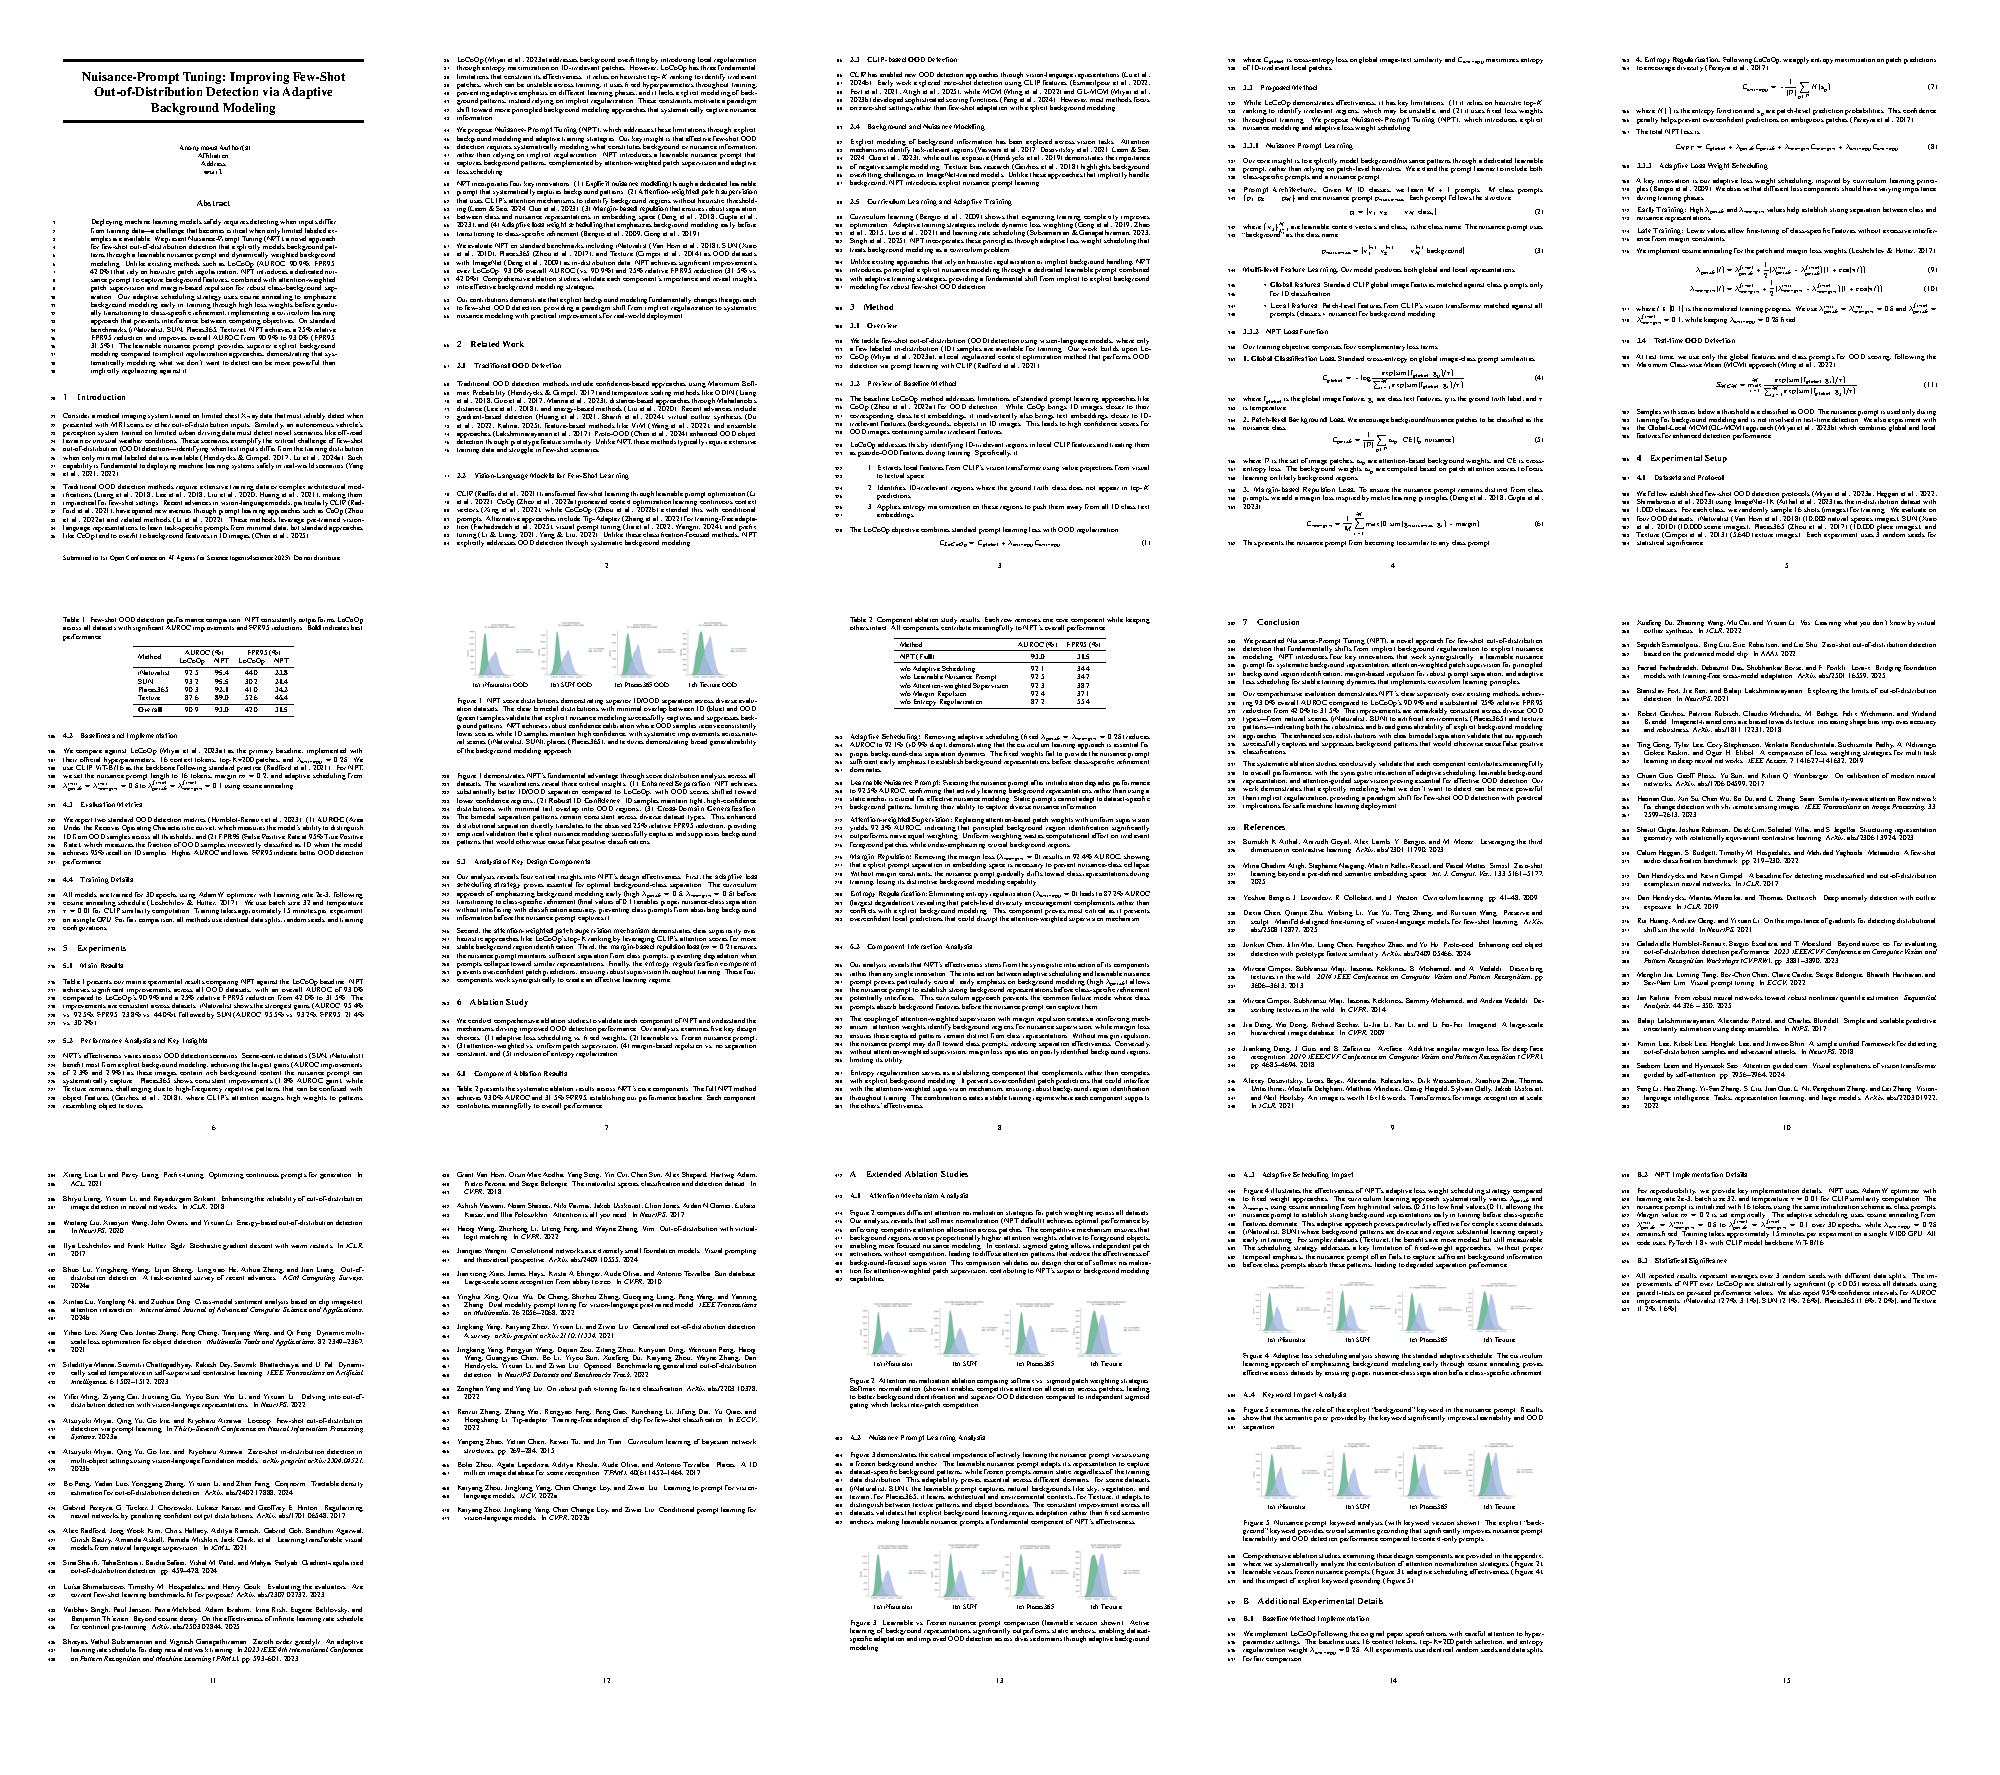
\includegraphics{images/paper_example.pdf}
    }
    \caption{An example of a generated paper. Our Jr. AI Scientist can generate full-length research papers with appendices.}
    \label{Fig:generated_paper}
\vspace{-2em}
\end{figure*}


\subsection{Results with Public AI Reviewers}

\begin{table*}[t]
\centering
\footnotesize
\caption{
Evaluation of AI-generated papers produced by various AI Scientist systems.
Scores represent the ratings given by DeepReviewer-14B~\citep{zhu2025deepreview} across public papers.
}
\label{tab:ai_scientist_combined}
\vspace{5pt}
\begin{subtable}[t]{1.0\textwidth}
\centering
\caption{Overall Score}
\begin{adjustbox}{width=\textwidth}
\begin{tabular}{lccccc}
\toprule
\textbf{AI Scientist Systems} & \textbf{Number}  & \textbf{Soundness} & \textbf{Presentation} & \textbf{Contribution} & \textbf{Rating} \\
\midrule
\textsc{AI Scientist-v1} & 10  & 2.03 & 2.05 & 1.83 & 3.30\\
AI Researcher & 7 & 1.86 & 1.79 & 1.79 & 3.25\\
\textsc{AI Scientist-v2} & 3 & 1.67 & 1.50 & 1.58 & 2.75 \\
CycleResearcher-12B & 6  & 2.25 & 2.25 & 2.04 & 3.92\\
Zochi & 2  & 2.50 & \textbf{2.75} & 2.38 & 4.50 \\
Jr. AI Scientist (Ours) & 3  & \textbf{2.75} & \textbf{2.75} & \textbf{2.75} & \textbf{5.75} \\
\bottomrule
\end{tabular}
\end{adjustbox}
\end{subtable}
\hfill
\\
\begin{subtable}[t]{1\textwidth}
\centering
\caption{Score for the Max Rating Paper}
\begin{adjustbox}{width=\textwidth}
\begin{tabular}{lccccc}
\toprule
\textbf{AI Scientist Systems} & \textbf{Number}  & \textbf{Soundness} & \textbf{Presentation} & \textbf{Contribution} & \textbf{Rating}\\
\midrule
\textsc{AI Scientist-v1} & 10  & 2.25 & 2.50 & 2.25 & 4.25 \\
AI Researcher & 7 & 2.25 & 2.25 & 2.00 & 4.25\\
\textsc{AI Scientist-v2} & 3 & 1.75 & 1.75 & 1.75 & 3.25 \\
CycleResearcher-12B & 6  & 2.75 & 2.75 & 2.75 & 5.00\\
Zochi & 2  & 2.50 & \textbf{3.00} & 2.50 & 5.00 \\
Jr. AI Scientist (Ours) & 3  & \textbf{3.00} & \textbf{3.00} & \textbf{3.00} & \textbf{6.25} \\
\bottomrule
\end{tabular}
\end{adjustbox}
\end{subtable}
\hfill
\\
\begin{subtable}[t]{1\textwidth}
\centering
\caption{Score for the Minimum Rating Paper}
\begin{adjustbox}{width=\textwidth}
\begin{tabular}{lccccc}
\toprule
\textbf{AI Scientist Systems} & \textbf{Number}  & \textbf{Soundness} & \textbf{Presentation} & \textbf{Contribution} & \textbf{Rating}\\
\midrule
\textsc{AI Scientist-v1} & 10  & 1.75 & 1.25 & 1.75 & 2.00\\
AI Researcher & 7 & 1.25 & 1.00 & 1.25 & 2.50 \\
\textsc{AI Scientist-v2} & 3 & 1.50 & 1.50 & 1.50 & 2.50  \\
CycleResearcher-12B & 6  & 2.00 & \textbf{2.50} & 1.50 & 3.00\\
Zochi & 2  & \textbf{2.50} & \textbf{2.50} & 2.25 & 4.00 \\
Jr. AI Scientist (Ours) & 3  & \textbf{2.50} & \textbf{2.50} & \textbf{2.50} & \textbf{5.00} \\
\bottomrule
\end{tabular}
\end{adjustbox}
\end{subtable}
\label{table:ai_reviewer_score}
\end{table*}


\textbf{Comparison Methods.}
As comparison methods, we used papers generated by existing AI Scientist systems.
Specifically, we included AI Scientist-v1~\citep{lu2024ai}, AI Scientist-v2~\citep{yamada2025ai}, AI-Researcher~\citep{tang2025ai}, CycleResearcher~\citep{weng2024cycleresearcher}, and Zochi~\citep{zochi2025}.

\textbf{Evaluation Metrics.}
For evaluation, we employed DeepReviewer~\citep{zhu2025deepreview}, an AI model designed to comprehensively assess research papers in a manner similar to expert reviewers. 
DeepReviewer is a 14B-parameter language model built by fine-tuning Phi-4 on the DeepReview-13K dataset, which contains structured, human-like review reasoning trajectories. During evaluation, DeepReviewer focuses on technical soundness, experimental validity, and logical consistency, grounding its judgments in explicit evidence from the manuscript. This design enables efficient and reliable evaluation while maintaining strong alignment with human reviewer judgments.
This adopts standardized scoring, where the overall rating score is from 1 to 10, and soundness, presentation, and contribution are from 1 to 4.
Compared to existing AI reviewers~\citep{weng2024cycleresearcher, lu2024ai, yamada2025ai}, DeepReviewer exhibits substantially stronger alignment with human reviewer evaluations, enabling efficient and reliable assessment of AI-generated paper reviews.
For the implementation, we utilize a single A100 80G GPU.

\textbf{Results.}
We evaluated papers generated by our system (an extension paper of LoCoOp is shown in \Cref{Fig:generated_paper}).
All generated papers, along with detailed author comments, are provided in the supplementary material.
We present our experimental results in \Cref{table:ai_reviewer_score}.
Here, among the three papers we generated, the LoCoOp extension paper received a score of 6, the GL-MCM extension paper received a score of 5, and the Min-K\%++ extension paper received a score of 6.25.
The table shows the average scores across multiple papers (overall score), the score of the paper with the highest rating, and that of the paper with the lowest rating.
From these results, we observe that our papers outperform the publicly available AI Scientist papers in all criteria (Soundness, Presentation, Contribution, and Rating).


\textbf{Score Distribution among Generated Papers.}
\Cref{Fig:score_distribution} shows the score distribution among all our generated papers before the author selection.
First, the average score over all 18 papers is 5.30. Although this is lower than the score of 5.75 reported in \Cref{table:ai_reviewer_score}, it can still be considered higher than those of existing AI-generated papers.
Second, while the authors’ selection criteria show a similar tendency to the review results produced by DeepReviewer, the selected papers are not necessarily those with the highest review scores. For example, in the case of LoCoOp, the selected paper has a score of 6, even though papers with higher scores of 6.25 and 6.50 exist. Upon manually reviewing these higher-scoring papers, we found that they contain more hallucinations in terms of numerical values and claims (Detailed hallucinations and risks are discussed in \Cref{sec:author_evaluation} and \Cref{sec:risk}. ).
These findings indicate that evaluation based solely on review scores is insufficient, and highlight the importance of author inspection and honest reporting of hallucinations and associated risks.

\begin{figure*}[t]
    \centering
    \resizebox{\textwidth}{!}{%
    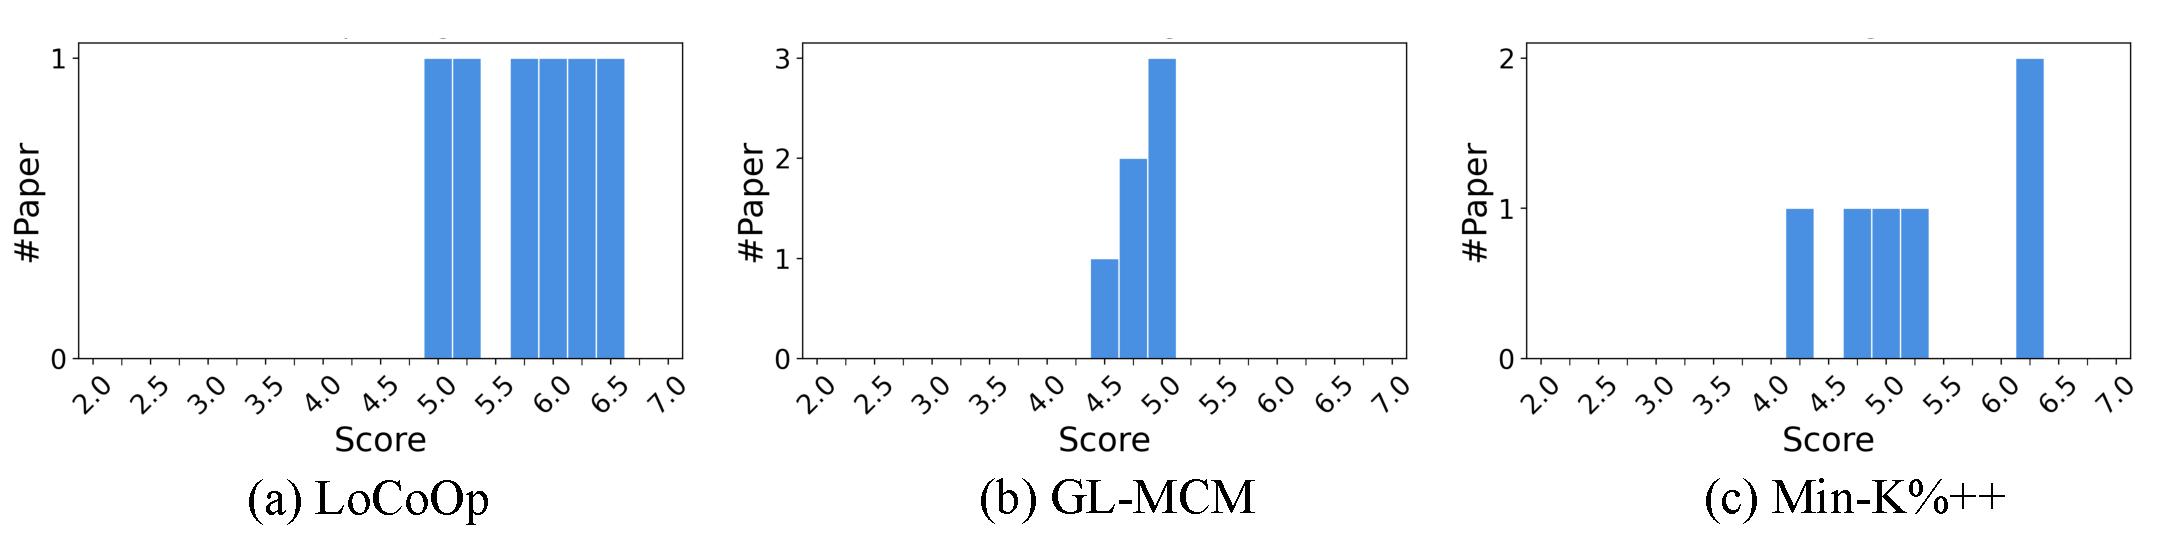
\includegraphics{images/paper_distribution.pdf}
    }
    \caption{A score distribution among all our generated papers before the author selection.}
    \label{Fig:score_distribution}
\vspace{-2em}
\end{figure*}